%\documentclass[a4paper]{article}
\usepackage[utf8]{inputenc}
\usepackage[spanish, es-tabla, es-noshorthands]{babel}
\usepackage[table,xcdraw]{xcolor}
\usepackage[a4paper, footnotesep = 1cm, width=22cm, top=2.5cm, height=25cm, textwidth=20cm, textheight=25cm]{geometry}
%\geometry{showframe}

\usepackage{tikz}
\usepackage{amsmath}
\usepackage{amsfonts}
\usepackage{amssymb}
\usepackage{float}
\usepackage{graphicx}
\usepackage{caption}
\usepackage{subcaption}
\usepackage{multicol}
\usepackage{multirow}
\usepackage{wrapfig}
\setlength{\doublerulesep}{\arrayrulewidth}
\usepackage{booktabs}

\usepackage{hyperref}
\hypersetup{
    colorlinks=true,
    linkcolor=blue,
    filecolor=magenta,      
    urlcolor=blue,
    citecolor=blue,    
}

\newcommand{\note}[1]{
	\begin{center}
		\huge{ \textcolor{red}{#1} }
	\end{center}
}

\setcounter{topnumber}{2}
\setcounter{bottomnumber}{2}
\setcounter{totalnumber}{4}
\renewcommand{\topfraction}{0.85}
\renewcommand{\bottomfraction}{0.85}
\renewcommand{\textfraction}{0.15}
\renewcommand{\floatpagefraction}{0.8}
\renewcommand{\textfraction}{0.1}
\setlength{\floatsep}{5pt plus 2pt minus 2pt}
\setlength{\textfloatsep}{5pt plus 2pt minus 2pt}
\setlength{\intextsep}{5pt plus 2pt minus 2pt}

\newcommand{\quotes}[1]{``#1''}
\usepackage{array}
\newcolumntype{C}[1]{>{\centering\let\newline\\\arraybackslash\hspace{0pt}}m{#1}}
\usepackage[american]{circuitikz}
\usetikzlibrary{calc}
\usepackage{fancyhdr}
\usepackage{units} 

\graphicspath{{../Ejercicio-1/}{../Ejercicio-2/}{../Ejercicio-3/}{../Ejercicio-4/}{../ParteI/}{../ParteII/}{../ParteIII/}{../ParteIV/}}

\pagestyle{fancy}
\fancyhf{}
\lhead{22.14 - Electrónica IV}
\rhead{Mechoulam, Lambertucci, Londero}
\rfoot{Página \thepage}

%
%\begin{document}

\subsection{Matrices de estado}

Para obtener teóricamente la transferencia del circuito, se vale del método de variables de estado. De esta forma, se llega a las siguientes matrices:

\begin{multicols}{2}
\begin{equation}
\mathbb{A} = 
\begin{pmatrix}
-\frac{DR_1}{L_1} + \frac{(1 - D) n^2 R_C R}{(R - R_C) L_1} & \frac{(1-D) n R}{(R - R_C) L_1}\\
-\frac{(1 - D) n R}{(R - R_C) C} & -\frac{D }{(R - R_C) C} - \frac{(1 - D)}{(R - R_C) C}
\end{pmatrix}
\end{equation}

\begin{equation}
\mathbb{B} = 
\begin{pmatrix}
	-\frac{D}{L_1} & 0\\
	0 & 0
\end{pmatrix}
\end{equation}

\begin{equation}
\mathbb{C} = 
\begin{pmatrix}
	-\frac{(1-D)n R R_C}{R - R_C} & \frac{D R}{R + R_C} + \frac{(1-D) R}{R - R_C}
\end{pmatrix}
\end{equation}

\begin{equation}
\mathbb{D} = 
\begin{pmatrix}
	0 & 0
\end{pmatrix}
\end{equation}
\end{multicols}

Se toman los valores seleccionados en la Sección (\ref{sec:parteii}). Además se consideran las resistencias tanto de $N_1$ y de los capacitores de salida (para las cuentas se consideran los dos capacitores en paralelo como uno solo con una única ESR) siendo estos $R_L = 0.001 \ \Omega$ y $R_C = 0.001 \ \Omega$ respectivamente. De esta forma se obtiene la transferencia del sistema:
\begin{equation}
	G(s) = \mathbb{C} \left(s \mathbb{I} - \mathbb{A} \right)^{-1} \mathbb{B} = \frac{-15.75 s + 3.351 \cdot 10^{8}}{s^2 + 3002s + 2.346 \cdot 10^{9}}
\end{equation}

\subsection{Compensador}

Se utiliza el siguiente circuito como compensador:
\begin{figure}[H]
	\centering
	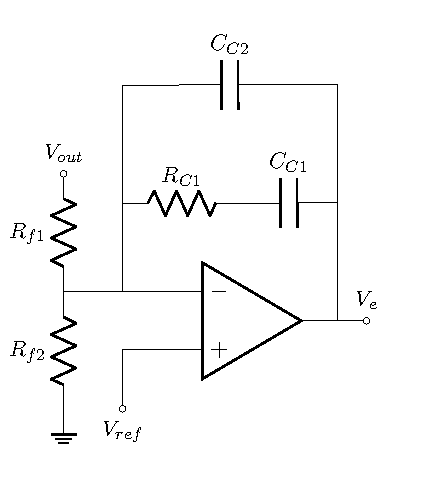
\includegraphics[width=0.3\linewidth, page = 1]{ImagenesParteIII/CircuitsP3.pdf}
	\label{fig:compensador}
	\caption{Circuito compensador del sistema.}
\end{figure}

La transferencia de este sistema es la siguiente:
\begin{equation}
	H(s) = \frac{ 1 }{ R_{f1} C_{C2} } \cdot \frac{s + \frac{1}{ R_{C1} C_{C1}}}{ s \left( s + \frac{R_{C1} + R_{C2}}{R_{C1} C_{C1} C_{C2}} \right)}
\end{equation}

Se emplean los siguientes valores:
\begin{multicols}{2}
\begin{itemize}
	\item $R_{C1} = 10 \ k\Omega$
	\item $R_{f1} = R_{f2} = 1 \ k\Omega$
	\item $C_{C1} = 10 \ nf$
	\item $C_{C2} = 1 \ \mu f$
	\item $N_2 = 1 \ \mu H$
\end{itemize}
\end{multicols}

Con esos valores, el compensador queda:
\begin{equation}
	H(s) = \frac{0.0001 s + 1}{ 1 \cdot 10^{-7} s^2 + 0.00101 s }
\end{equation}

De esta forma, la ganancia de lazo queda de la forma:
\begin{equation}
	T(s) = G(s) \cdot H(s) = \frac{-0.001575 s^2 + 3.35 \cdot 10^4 s + 3.351 \cdot 10^8}{ 1 \cdot 10^{-7} s^4 + 0.00131 s^3 + 237.6 s→^2 + 2.369 \cdot 10^6 s }
\end{equation}

Con el sistema realimentado, se grafican los diagramas de Bode para la transferencia y para la ganancia de lazo T, algiual que el diagrama de polos y ceros del sistema.
\begin{figure}[H]
	\centering
	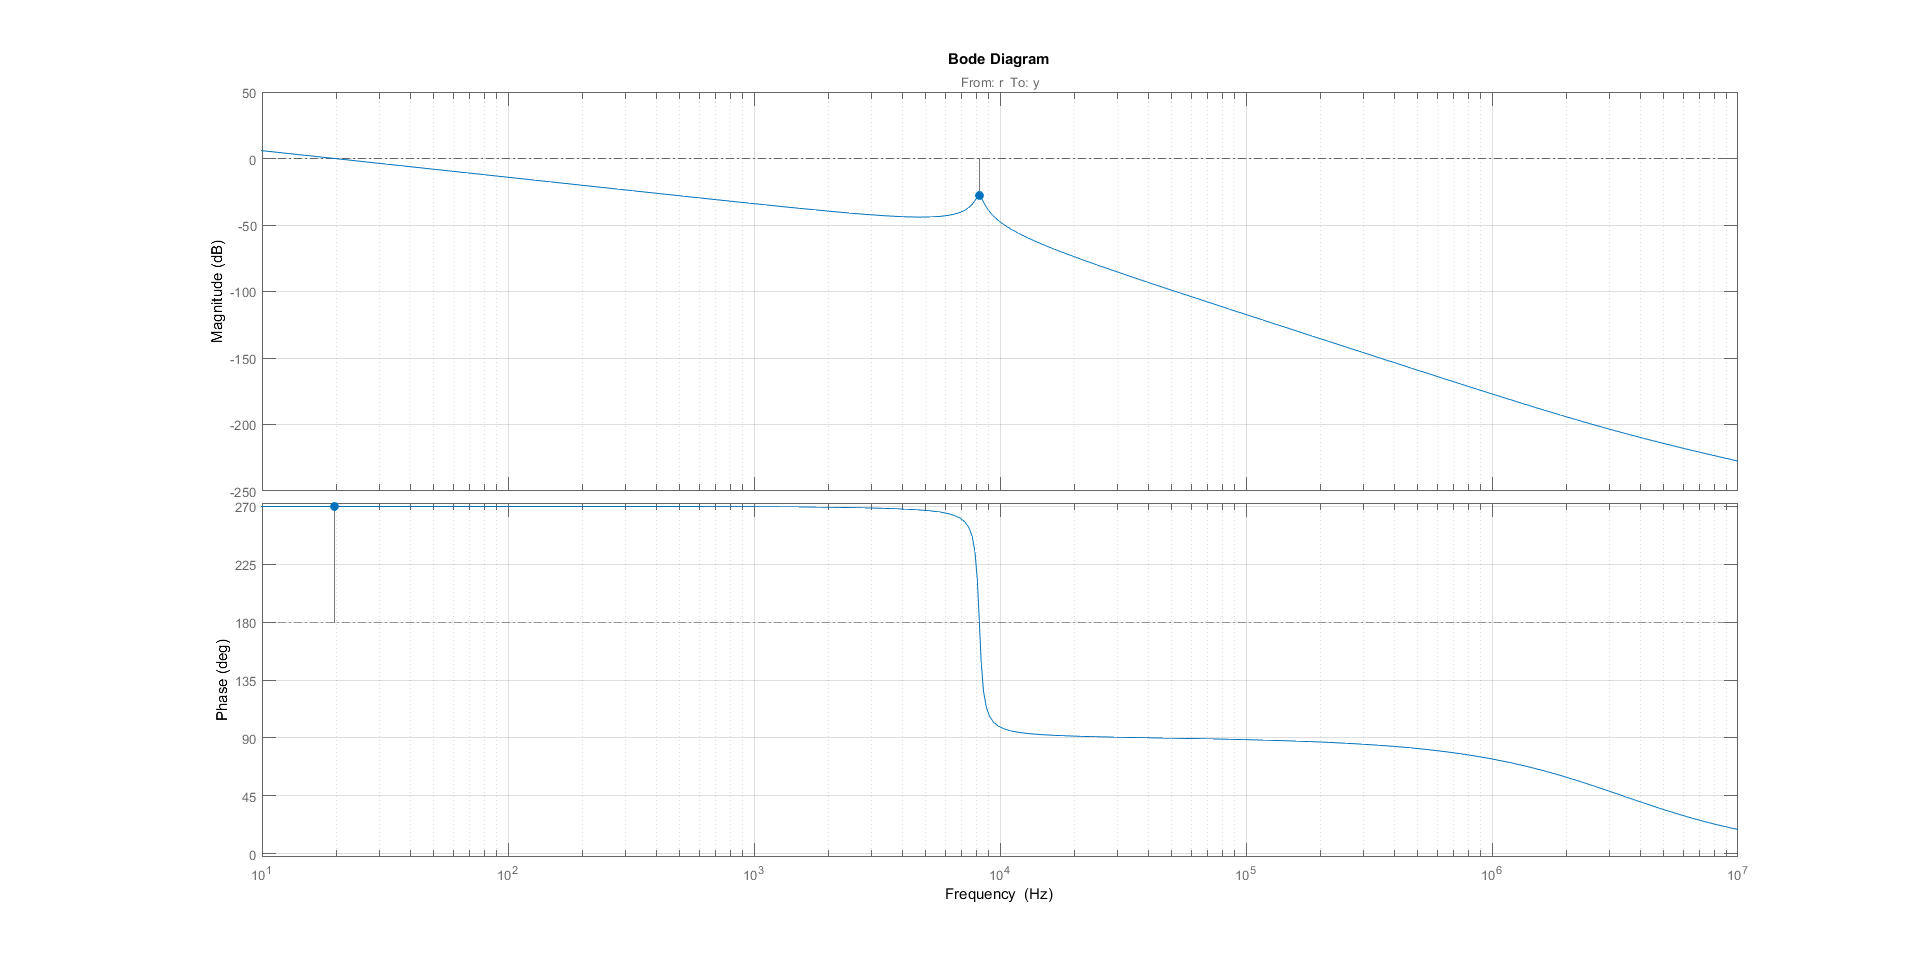
\includegraphics[width=0.8\linewidth]{ImagenesParteIII/Bode.png}
	\label{fig:bode}
	\caption{Diagrama de Bode transferencia.}
\end{figure}
\begin{figure}[H]
	\centering
	\includegraphics[width=0.8\linewidth]{ImagenesParteIII/BodeT.png}
	\caption{Diagrama de Bode ganancia de lazo.}
	\label{fig:bodeT}
\end{figure}

\begin{figure}[H]
	\centering
	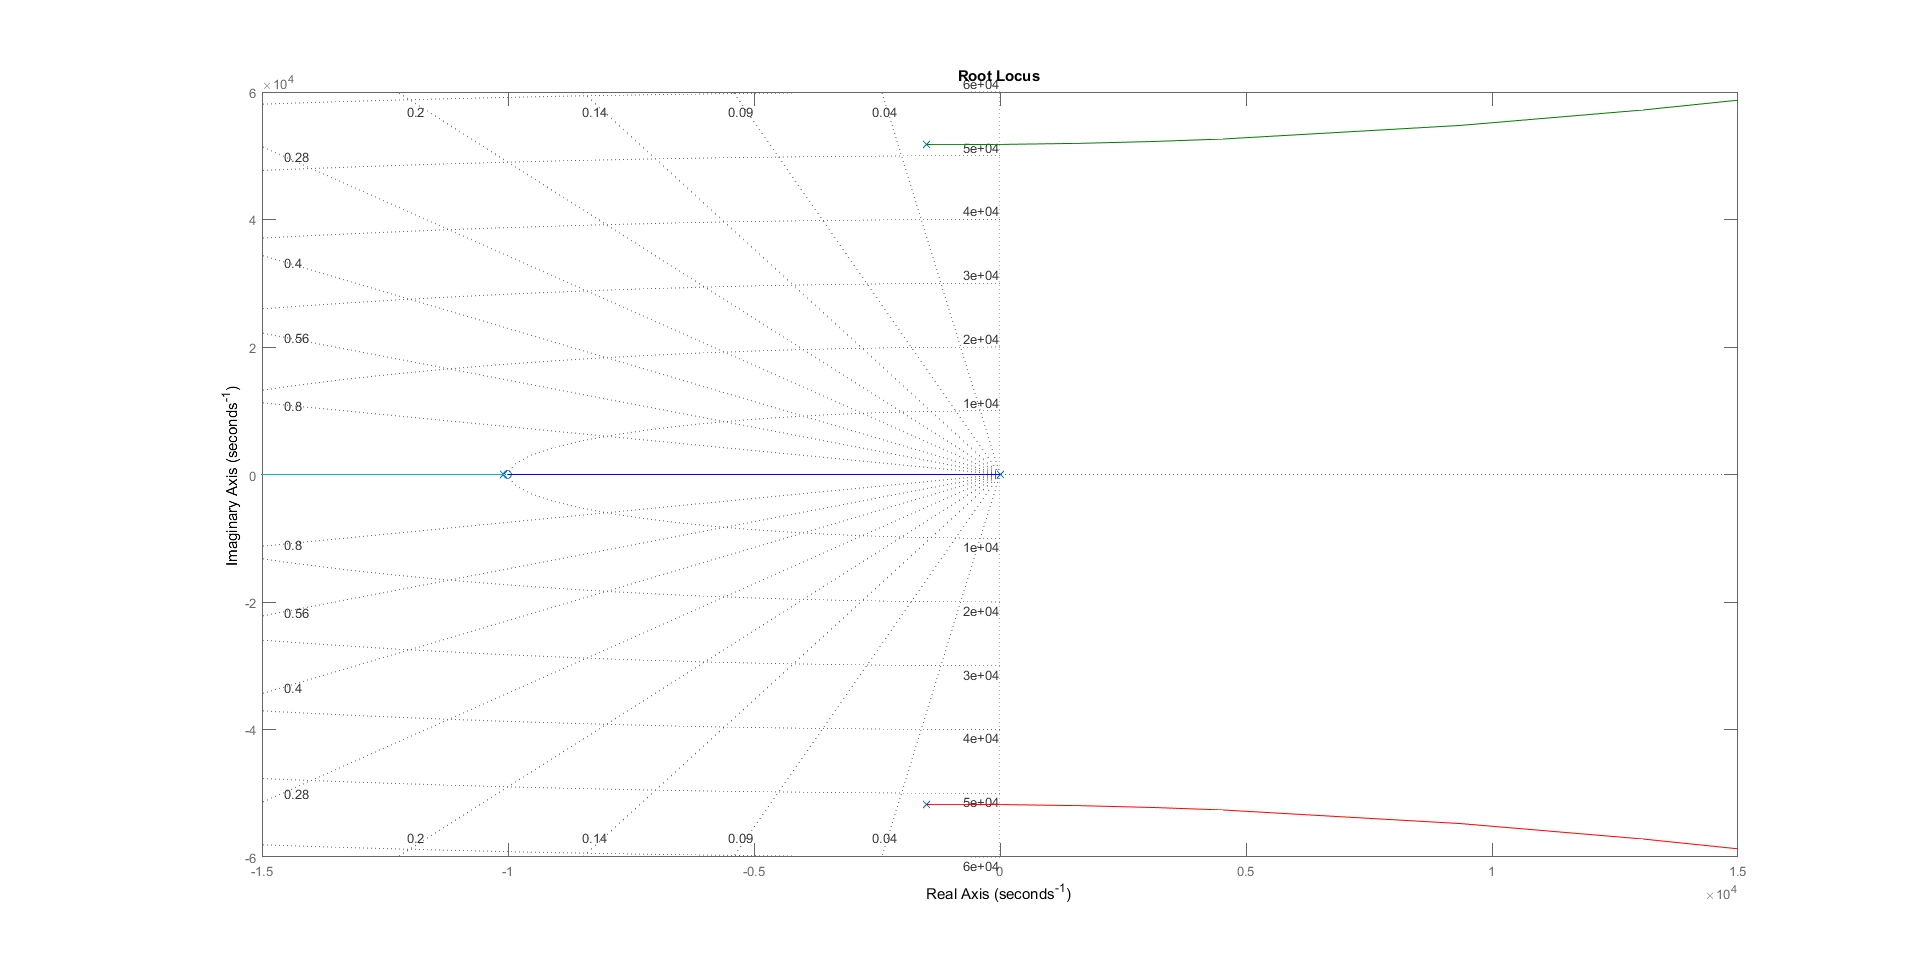
\includegraphics[width=0.8\linewidth]{ImagenesParteIII/Rlocus.png}
	\label{fig:zplane}
	\caption{Plano S, diagrama de polos y ceros.}
\end{figure}
Una particualridad de la topología Flyback es la existencia de un cero en el semiplano derecho.\\
En lineas generales, si 
\begin{equation}
|T| >> 1 \implies \ \frac{V_o}{V_{ref}} \approx \frac{1}{\beta} = 2 \ \implies V_o\approx 2\cdot V_{ref} 
\end{equation}

En el diseño del realimentador se tuvieron en cuenta diversos lugares para colocar una resistencia variable. Esta podría ser en $R_{f1}$, $R_{f2}$ o simplemente se podría variar la $V_{ref}$.

El problema que se encontró con poner la variable en $R_{f2}$ es que la variación de salida con esta resistencia resulta homográfica, siendo preferible que sea lineal. Es por ello que esta opción quedó descartada. Finalmente se optó por variar únicamente la tension de $V_{ref}$.

Debido a que los potenciómetros cuentan con una inductancia parásita considerable y, dado que este es el realimentador, se podrían introducir polos ó ceros indeseados al sistema empleando dicho componente.
 \subsection{Simulaciones}
Finalmente se realizó la simulación a lazo cerrado y se obtuvieron las siguientes curvas:

\begin{figure}[H]
	\centering
	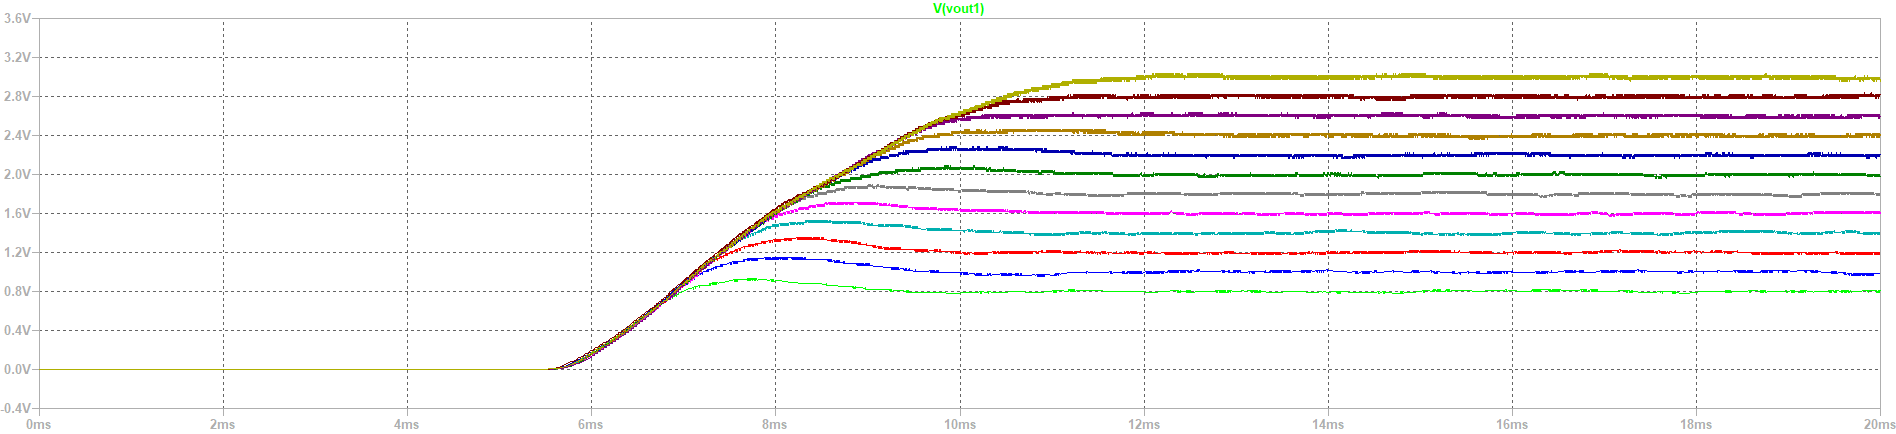
\includegraphics[width=0.9\linewidth]{ImagenesParteIII/Vouts.png}
	\label{fig:vouts_3}
	\caption{Variación de tensión de salida.}
\end{figure}
Al igual se midieron todas las curvas relevantes del sistema:

En el caso de la tensión de salida, se observa un ripple del 2\%.
\begin{figure}[H]
	\centering
	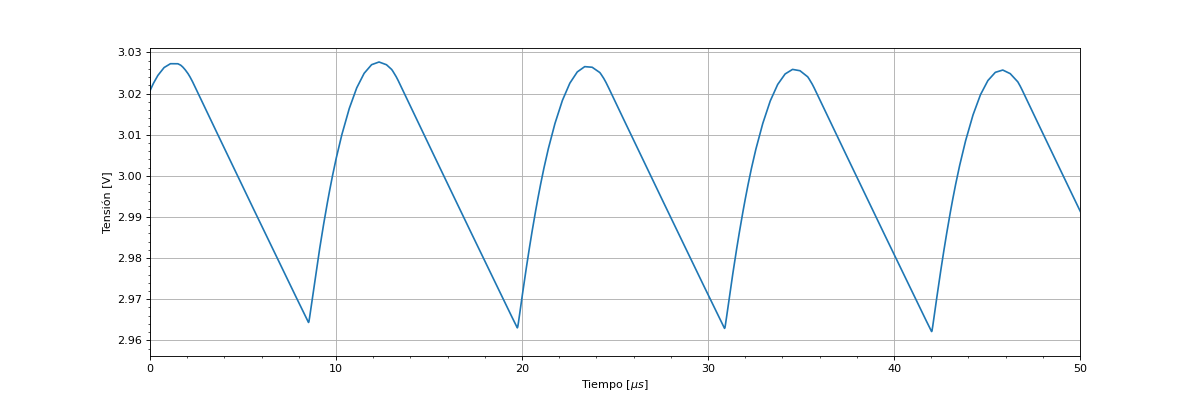
\includegraphics[width=\linewidth]{ImagenesParteIII/Vo.png}
	\label{fig:voIII}
	\caption{Tensión de salida.}
\end{figure}

\begin{figure}[H]
	\centering
	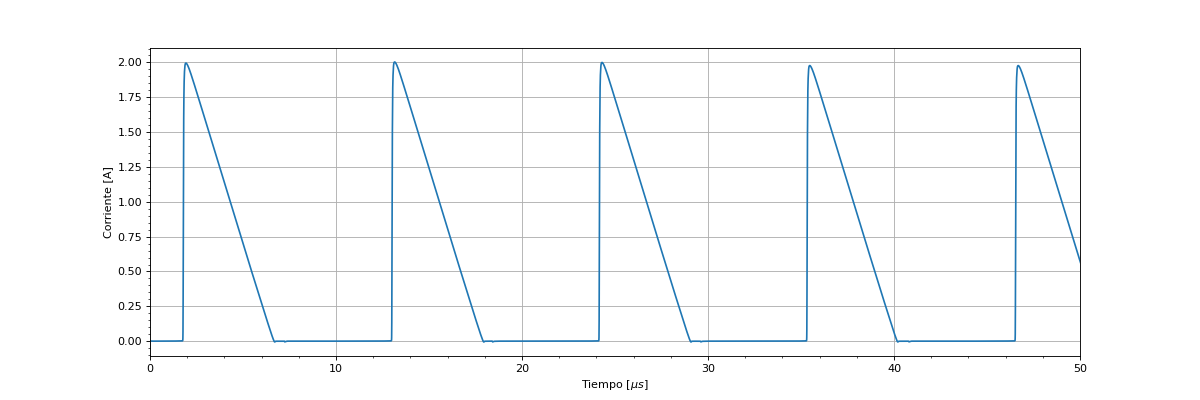
\includegraphics[width=\linewidth]{ImagenesParteIII/Idiodo.png}
	\label{fig:idiodoIII}
	\caption{Corriente del diodo.}
\end{figure}

Se puede observar en esta simulación y todas las siguientes, que se produce una pequeña oscilación proveniente del nodo de switching, la cual se propaga al resto del circuito mediante la relación de transformación. El origen de estas oscilaciones se debe a la pérdida de energía total en el campo magnético del transformador la cual antes provocaba que se polarice el diodo del secundario en directa. Al acabarse la energía del núcleo y polarizándose débilmente al diodo en inversa, circula la corriente de reverse recovery del diodo por el secundario, inyectándose por la relación de transformación al primario, y finalmente produciendo oscilaciones entre la inductancia del primario y la capacitancia de salida del transistor.

\begin{figure}[H]
	\centering
	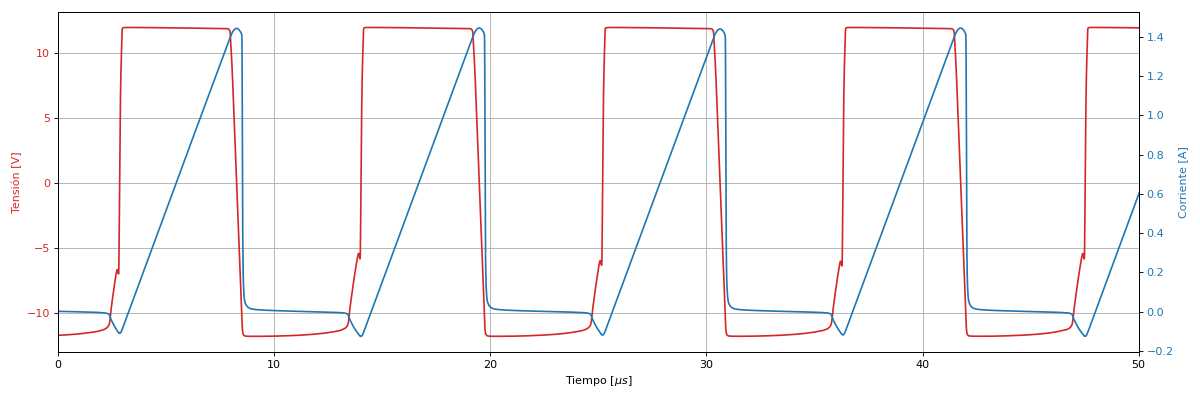
\includegraphics[width=0.9\linewidth]{ImagenesParteIII/Primario.png}
	\caption{Tensión y corriente del primario.}
	\label{fig:primarioIII}

\end{figure}

\begin{figure}[H]
	\centering
	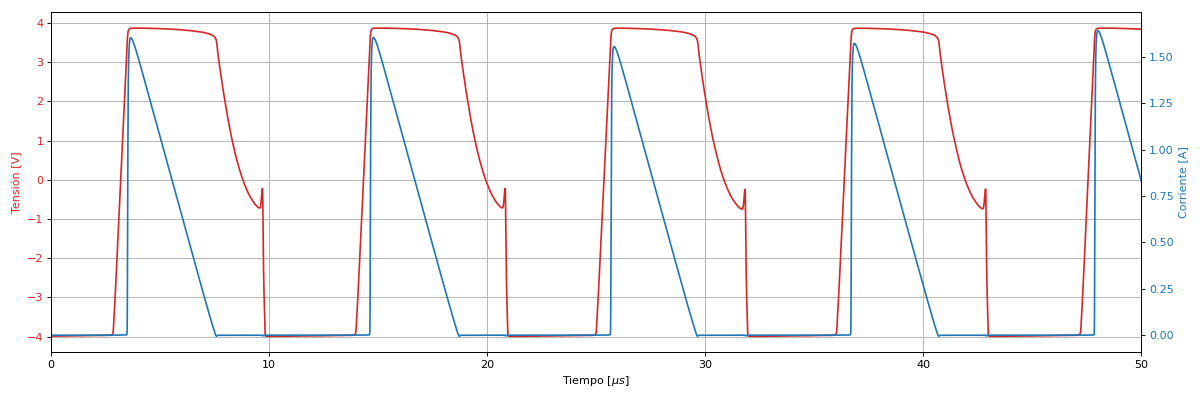
\includegraphics[width=0.9\linewidth]{ImagenesParteIII/Secundario.png}
	\label{fig:secundarioiii}
	\caption{Tensión y corriente del secundario.}
\end{figure}
Aqui se ve la tensión de compensación del SG3525 realimentado.
\begin{figure}[H]
	\centering
	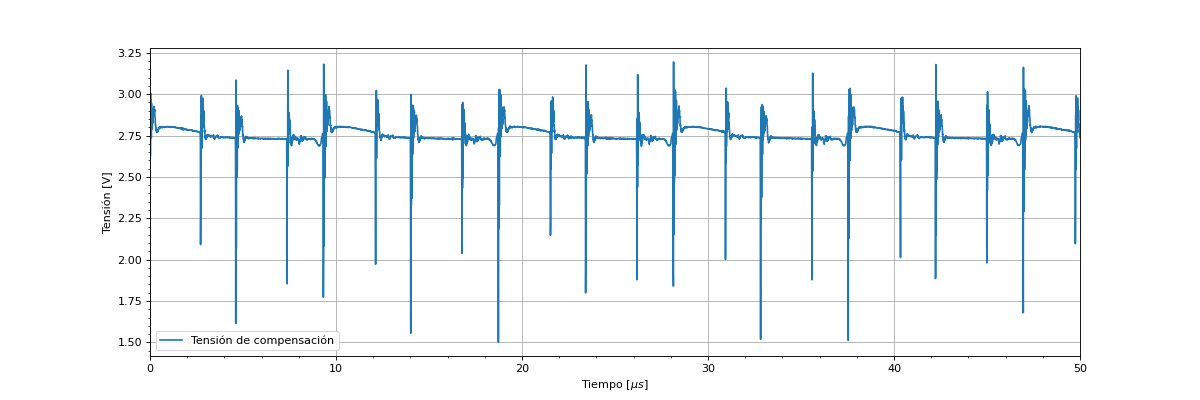
\includegraphics[width=0.9\linewidth]{ImagenesParteIII/Vcom.png}
	\caption{Tensión de compensación.}
	\label{fig:com3}

\end{figure}

\begin{figure}[H]
	\centering
	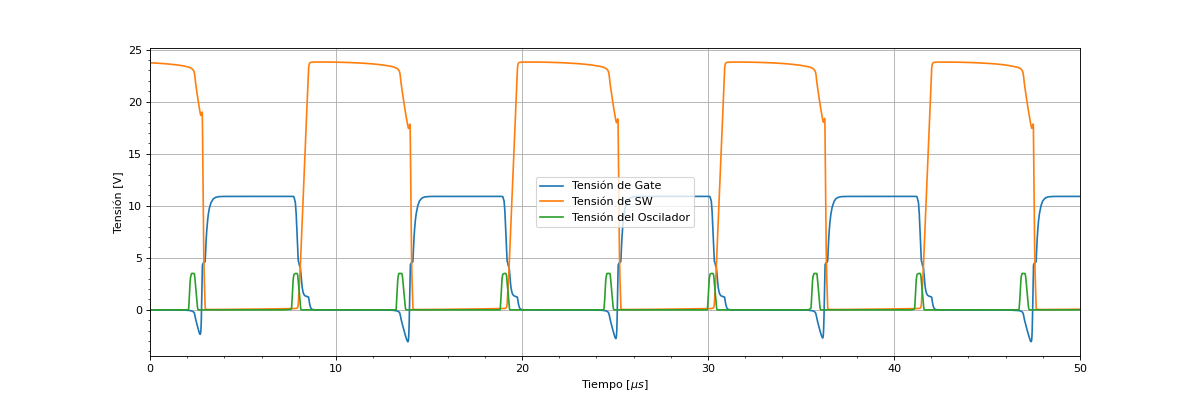
\includegraphics[width=\linewidth]{ImagenesParteIII/TensionesVarias1.png}
	\label{fig:tensionesvarias}
	\caption{Tensión de Gate y del Switch.}
\end{figure}
\begin{figure}[H]
	\centering
	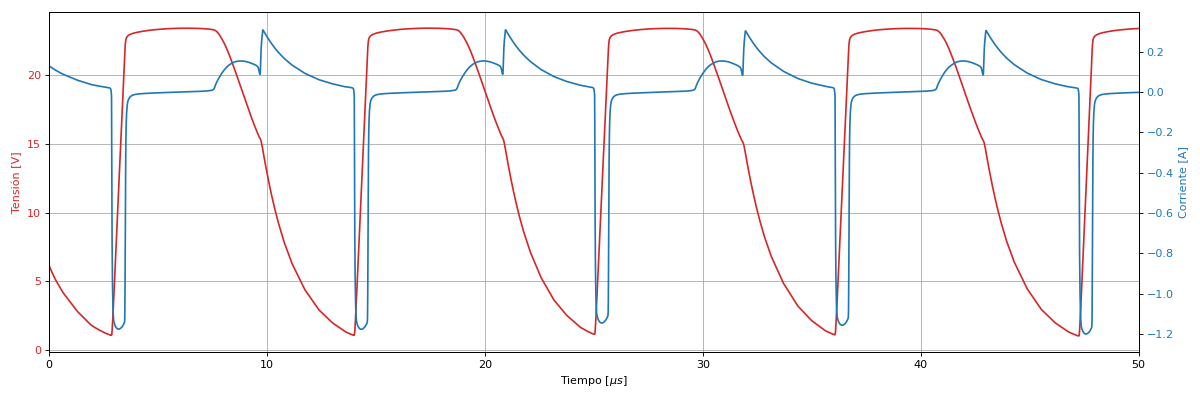
\includegraphics[width=0.9\linewidth]{ImagenesParteIII/Cap_snub.png}
	\label{fig:tensionsVsnubIII}
	\caption{Tensión y corriente en el capacitor de snubber.}
\end{figure}
También se colocó en la simulación varios capacitores en paralelo con varias ESR distintas ($10m\Omega \sim 1 \Omega$). Se observa el efecto característico de la ESR sobre la tensión de salida provocando "saltos" de tensión sobre la misma como se ve a continuación.
\begin{figure}[H]
	\centering
	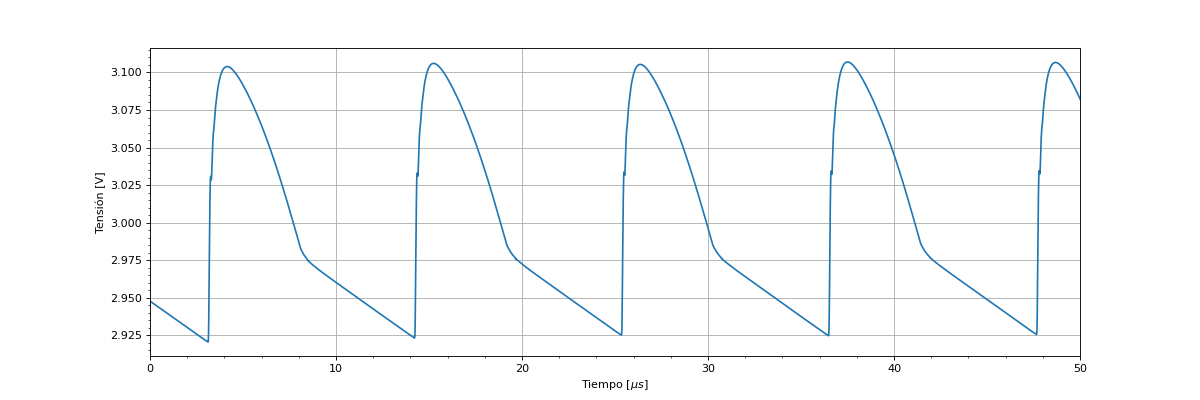
\includegraphics[width=0.9\linewidth]{ImagenesParteIII/Vout_esr.png}
	\label{fig:tensionESR}
	\caption{Tensión de salida con ESR.}
\end{figure}
Esto se puede subsanar al agregar aun mas capacitores en paralelo que reduzcan la ESR.

Finalmente vale la pena mencionar la desaparición casi completa de las grandes oscilaciones que se observaban en la sección anterior, esto se debe a la introducción del circuito de snubber.

%\end{document}